\section{Background}\label{sec:background}

\textbf{Homepage2Vec} addresses the limitations of existing approaches to web page representation by introducing a multilingual, embeddings-based model. Prior to its development, no multilingual models or widely adopted embedding-based methods existed for web page analysis, often necessitating the use of paid services. Homepage2Vec revolutionizes this landscape by providing a multilingual, open-source solution based on embeddings. Additionally, the model is efficient, enabling local execution without external APIs, ensuring accessibility and speed for a diverse range of users.

\texttt{Homepage2Vec} is trained on a publicly available website directory and corresponding labels called Curlie, maintained by a volunteer community. The directory comprises 3 million websites in 92 languages, labeled in hierarchical categories. After removing duplicates and retaining accessible sites, the dataset contains 886K entries. For classification, only top-level labels are considered, resulting in 14 classes.  The label distribution is imbalanced, with most websites categorized as Business (27\%), followed by Society (13.9\%) and Arts (9\%). The dataset is primarily single-labeled, with only 2.1\% of samples appearing in two or more taxonomy trees of the 14 top-level classes \cite{homepage2vec}.
% The majority of websites are in English (40\%), followed by German (16\%), French (5\%), and Japanese (6\%).

The model, after scraping a website's homepage, parses the raw HTML and URL into a one-dimensional embedding. Specifically, \textit{url}, \textit{title}, \textit{description}, \textit{keywords}, \textit{links}, and \textit{sentences} are embedded via the multilingual model XLM-R \cite{xmlr}, while \textit{tld} and \textit{metatags} are one-hot encoded based on a predefined list of the most common top-level domains (excluding regional ones) and meta-tags. For features resulting in multiple embeddings, such as sentences, the mean is taken. Finally, all embeddings are concatenated, resulting in an input dimension of $4665$. The resulting embedding is then fed into a fully connected neural network with 2 hidden layers of sizes 1000 and 100, respectively, each followed by a ReLU activation function and dropout with a probability of $0.5$. Importantly, the outputs are treated separately, with each output transformed via sigmoid and interpreted as a probability for the given class.

\begin{figure}[!ht]
    \centering
    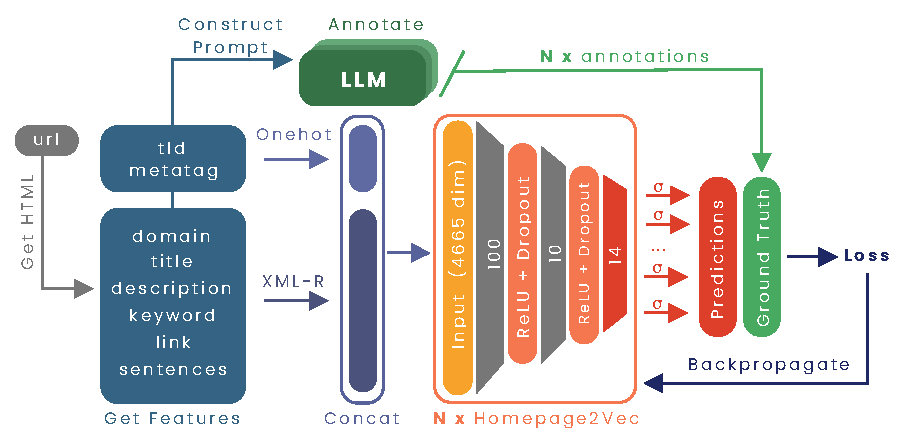
\includegraphics[height=0.2\textheight, width=\columnwidth]{./figures/training_overview.pdf}
    \caption{\textbf{Training overview.} Sth else}
    \label{fig:train-overview}
\end{figure}

Homepage2Vec, evaluated against an unbalanced Curlie test set, achieves a macro-averaged precision of $0.771$, recall of $0.549$, and an F1-score of $0.634$ \cite{homepage2vec}. While these results are promising, it is crucial to note that the majority of websites have at most one label. Therefore, the task is inherently easier than the one being addressed. To account for this, we evaluate the model on a crowdsourced dataset of 840 samples, where each website has an average of $2.5$ labels. We obtain a macro F1-score of $0.38$, serving as our baseline for further improvement using the proposed methods described in the following section.

% - GPT annotations 
\textbf{GPT-Based Labeling:} Utilizing GPT for streamlined annotation proves to be a powerful approach, as demonstrated in prior research \cite{reduce-labeling-cost, prompt-tuning, is-gpt3-good-annot, annollm}. While GPT-based labeling offers numerous advantages, relying on it for inference is suboptimal due to cost and time constraints, as suggested in previous work \cite{reduce-labeling-cost, is-gpt3-good-annot}. Instead, a more viable option is to employ GPT-generated labels for training a classifier, as pursued in this work. Additionally, our research extends beyond previous focuses on GPT-3, exploring the efficacy of GPT-4 for the same task. Finally, in contrast to prior studies, which focused solely on single-label classification with a limited number of classes \cite{reduce-labeling-cost, is-gpt3-good-annot}, our research expands the scope by investigating the effectiveness of GPT for multi-label classification tasks with $14$ possible classes.
